% File: backmatter/Appendix.tex
% Consolidated Appendices for the Thesis

\cleardoublepage
\appendix
\addcontentsline{toc}{chapter}{Appendices}  % Adds "Appendices" entry in TOC (optional but recommended)

\chapter{Feasibility Comparison Table}  % Automatically becomes "Appendix A: Feasibility Comparison Table"

\begin{table}[htbp]
    \centering
    \caption{Feasibility Comparison Table}
    \label{tab:feasibility}
    \vspace{1em}  % Space between caption and table
    \small  % Improves readability and fit
    \begin{adjustbox}{max width=\textwidth}  % Safely constrains to margins if needed
        \begin{tabular}{>{\raggedright\arraybackslash}p{3.2cm} >{\raggedright\arraybackslash}p{4.2cm} >{\raggedright\arraybackslash}p{6cm} >{\raggedright\arraybackslash}p{3.4cm}}
            \toprule
            \textbf{Feasibility Type} & \textbf{Description} & \textbf{Key Factors Considered} & \textbf{Conclusion} \\
            \midrule
            Technical Feasibility
            & Checks if the suggested technologies can be effectively put into use and combined with existing systems.
            & \begin{itemize}[nosep, left=1em, wide=0pt]
                \item Cloud computing allows for easy scaling and access to resources from anywhere.
                \item GPS and NFC technologies offer precise real-time tracking capabilities.
                \item AI-driven route optimization improves overall efficiency.
                \item Secure compatibility with current K-Electric systems is ensured.
            \end{itemize}
            & Feasible – The needed technology is already available, works well, and can be used with the organization's current systems. \\[8pt]
            
            Economic Feasibility
            & Checks if the project offers a good value for money and explains why the investment is worthwhile.
            & \begin{itemize}[nosep, left=1em, wide=0pt]
                \item Better route planning can save up to 15\% on fuel expenses.
                \item Using predictive maintenance helps cut down on equipment breakdowns and repair bills.
                \item Enhancing how operations run leads to higher levels of productivity.
            \end{itemize}
            & Feasible – The system will result in long-term cost savings, which makes the investment a good choice. \\[8pt]
            
            Cost Feasibility
            & Checks if the project's cost stays within the budget and can be maintained over a long period.
            & \begin{itemize}[nosep, left=1em, wide=0pt]
                \item The first expenses involve buying hardware like GPS and NFC devices, developing the software, and connecting everything together.
                \item Ongoing costs come from using cloud services, keeping the system running, and making regular updates.
                \item The return on investment happens because the system helps save time and lowers overall operating costs.
            \end{itemize}
            & Feasible – The project needs some initial spending, but the money saved on fuel, repairs, and better performance makes it a good choice for lasting success. \\
            \bottomrule
        \end{tabular}
    \end{adjustbox}
\end{table}

This comparison shows that the proposed Real-Time Fleet Tracking System works well from a technical, economic, and cost point of view. It ensures efficient, scalable, and cost-effective fleet management for K-Electric.

% Next appendices will be added here (e.g., \chapter{Title for Appendix B} ...)
% Appendix B: Additional References Consulted
\chapter{Additional References Consulted}

These sources were consulted during the literature review to support discussions on real-time fleet tracking benefits, response times, predictive maintenance, and security standards.

\begin{enumerate}
    \item Aberdeen Group. (2015). \textit{Improving Fleet Efficiency with Real-Time Tracking}.
    
    \item JIMI IoT. \textit{Boost Your Business with Real-Time Fleet Tracker}. Retrieved from: \url{https://www.jimiiot.com/news/boost-your-business-with-real-time-fleet-tracker.html}
    
    \item FieldLogix. \textit{Fleet Tracking Improves Customer Service via Better Response Times}. Retrieved from: \url{https://fieldlogix.com/news/fleet-tracking-improves-customer-service-via-better-response-times/}
    
    \item Fleetx. \textit{The Transformative Impact of Vehicle Tracking Solutions on Service and Satisfaction}. Retrieved from: \url{https://blog.fleetx.io/the-transformative-impact-of-vehicle-tracking-solutions-on-service-and-satisfaction/}
    
    \item GoFleet. (2021). \textit{How Real-Time GPS Tracking Improves Fleet Response Times}. Retrieved from: \url{https://www.gofleet.com/advantages-of-real-time-tracking/}
    
    \item FieldLogix. (2020). \textit{The Benefits of Fleet Tracking for Service Response Times}. Retrieved from: \url{https://www.fieldlogix.com}
    
    \item IETF. \textit{RFC 5246: The Transport Layer Security (TLS) Protocol Version 1.2}. Retrieved from: \url{https://datatracker.ietf.org/doc/html/rfc5246}
    
    \item NIST. \textit{FIPS PUB 197: Advanced Encryption Standard (AES)}. Retrieved from: \url{https://nvlpubs.nist.gov/nistpubs/FIPS/NIST.FIPS.197.pdf}
    
    \item Emerald Insight. Article on related fleet topics. Retrieved from: \url{https://www.emerald.com/insight/content/doi/10.1108/meq-07-2018-0134/full/html}
    
    \item Translogixs. \textit{How Predictive Maintenance Can Save Your Fleet Time and Money}. Retrieved from: \url{https://www.translogixs.com/blog-posts/how-predictive-maintenance-can-save-your-fleet-time-and-money}
    
    \item Fleet Owner. (n.d.). \textit{Fleets Save More with Predictive Maintenance}. Retrieved from: \url{https://www.fleetowner.com/technology/article/21260642/fleets-save-more-with-predictive-maintenance}
    
    \item Prolius. \textit{Predictive Maintenance}. Retrieved from: \url{https://www.prolius.com/news/predictive-maintenance}
\end{enumerate}


% Appendix C: Hardware Components Specifications and Pin Configurations
\chapter{Hardware Components Specifications and Pin Configurations}

This appendix provides detailed technical specifications, pin configurations, and logical diagrams for the key hardware components used in the project.

\section{ESP32-S3 Microcontroller}

\textbf{Technical Specifications}
\begin{itemize}
    \item Supply Voltage: 3.0V – 3.6V (typical 3.3V)
    \item CPU: Dual-core Xtensa LX7, 240 MHz
    \item RAM: 512 KB SRAM + external PSRAM support
    \item Flash: 8 MB (typical module)
    \item Communication Interfaces: UART, SPI, I2C, GPIO, PWM, ADC, DAC
    \item Wireless: Wi-Fi (2.4 GHz, 802.11 b/g/n), Bluetooth 5.0 LE
\end{itemize}

\textbf{Pin Configuration}

\begin{table}[htbp]
    \centering
    \caption{ESP32-S3 Microcontroller Pin Configuration}
    \label{tab:esp32_pins}
    \small
    \begin{tabular}{l l p{5cm} p{5cm}}
        \toprule
        \textbf{Pin No.} & \textbf{Name} & \textbf{Function} & \textbf{Connection in Project} \\
        \midrule
        1 & 3V3 & Power supply (3.3V) & Power regulator output \\
        2 & GND & Ground & Common ground \\
        3 & GPIO21 & I2C SDA & PN532 NFC SDA \\
        4 & GPIO22 & I2C SCL & PN532 NFC SCL \\
        5 & GPIO16 & UART RX & GPS TX \\
        6 & GPIO17 & UART TX & GPS RX \\
        7 & GPIO5 & SPI SCK & SD Card + LCD \\
        8 & GPIO18 & SPI MOSI & SD Card + LCD \\
        9 & GPIO19 & SPI MISO & SD Card \\
        10 & GPIO23 & UART TX & GSM RX (via level shifter) \\
        11 & GPIO25 & UART RX & GSM TX (via level shifter) \\
        \bottomrule
    \end{tabular}
\end{table}

\begin{figure}[htbp]
    \centering
    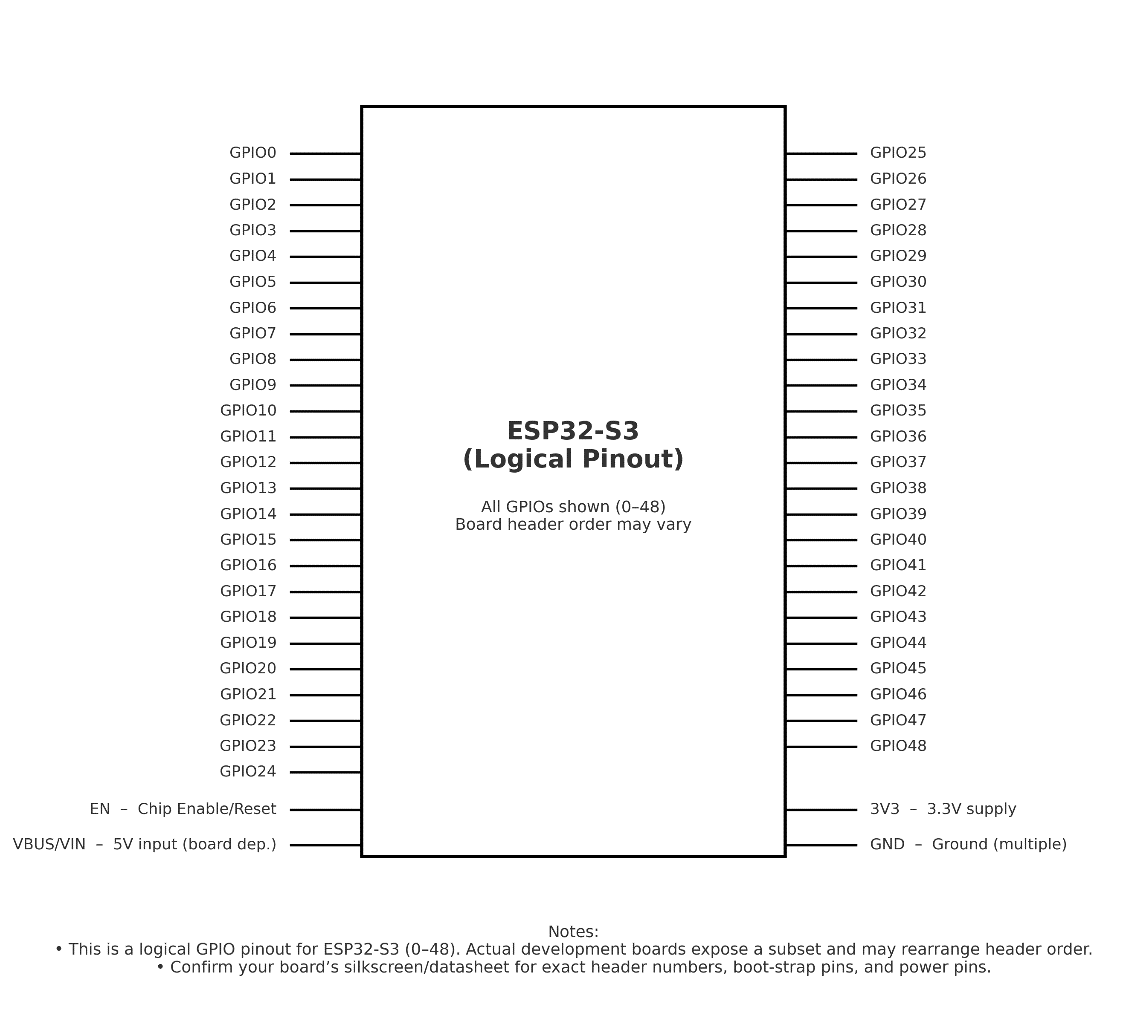
\includegraphics[width=\textwidth]{backmatter/figs/c1.png}  % Update path to actual file
    \caption{ESP32-S3 full logical pinout}
    \label{fig:esp32_pinout}
\end{figure}

\section{PN532 NFC Reader}

\textbf{Technical Specifications}
\begin{itemize}
    \item Operating Voltage: 3.3V / 5V
    \item Communication Interfaces: I2C, SPI, UART
    \item Frequency: 13.56 MHz
    \item Reading Range: 0–5 cm (depending on antenna \& card type)
\end{itemize}

\textbf{Pin Configuration}

\begin{table}[htbp]
    \centering
    \caption{PN532 NFC Reader Pin Configuration}
    \label{tab:pn532_pins}
    \small
    \begin{tabular}{l l p{5cm} p{5cm}}
        \toprule
        \textbf{Pin No.} & \textbf{Name} & \textbf{Function} & \textbf{Connection in Project} \\
        \midrule
        1 & VCC & Power & 3.3V \\
        2 & GND & Ground & Common ground \\
        3 & SDA & I2C Data & ESP32 GPIO21 \\
        4 & SCL & I2C Clock & ESP32 GPIO22 \\
        5 & IRQ & Interrupt Pin & Not used \\
        \bottomrule
    \end{tabular}
\end{table}

\begin{figure}[htbp]
    \centering
    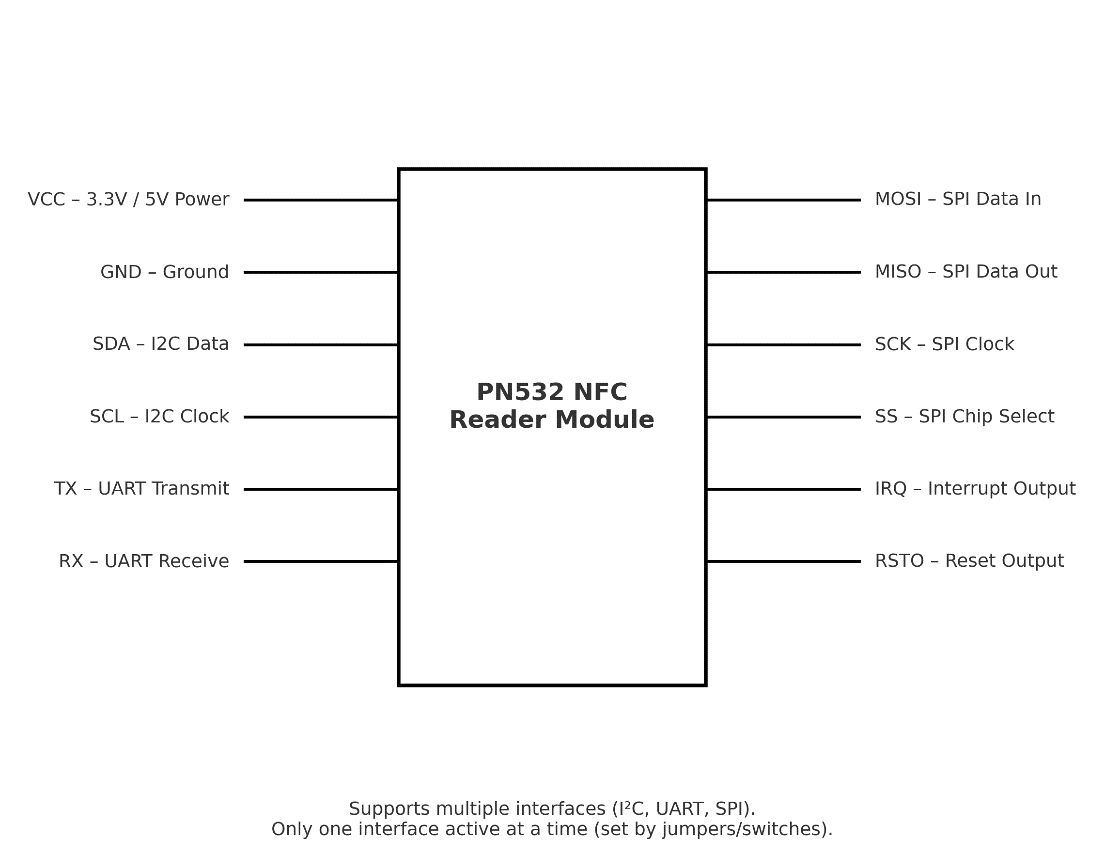
\includegraphics[width=0.8\textwidth]{backmatter/figs/c2.png}
    \caption{PN532 NFC Reader full logical pinout}
    \label{fig:pn532_pinout}
\end{figure}

\section{SIM900A GSM Module}

\textbf{Technical Specifications}
\begin{itemize}
    \item Operating Voltage: 3.4–4.4V (recommended 4V)
    \item Peak Current: 2A (during transmission bursts)
    \item Network: Quad-band GSM 850/900/1800/1900 MHz
    \item Interface: UART (AT commands)
\end{itemize}

\textbf{Pin Configuration}

\begin{table}[htbp]
    \centering
    \caption{SIM900A GSM Module Pin Configuration}
    \label{tab:sim900a_pins}
    \small
    \begin{tabular}{l l p{5cm} p{5cm}}
        \toprule
        \textbf{Pin No.} & \textbf{Name} & \textbf{Function} & \textbf{Connection} \\
        \midrule
        1 & VCC & Power 4V & External Regulator \\
        2 & GND & Ground & Common GND \\
        3 & TXD & UART Data Out & ESP32 RX25 (via level shifter) \\
        4 & RXD & UART Data In & ESP32 TX23 (via level shifter) \\
        \bottomrule
    \end{tabular}
\end{table}

\begin{figure}[htbp]
    \centering
    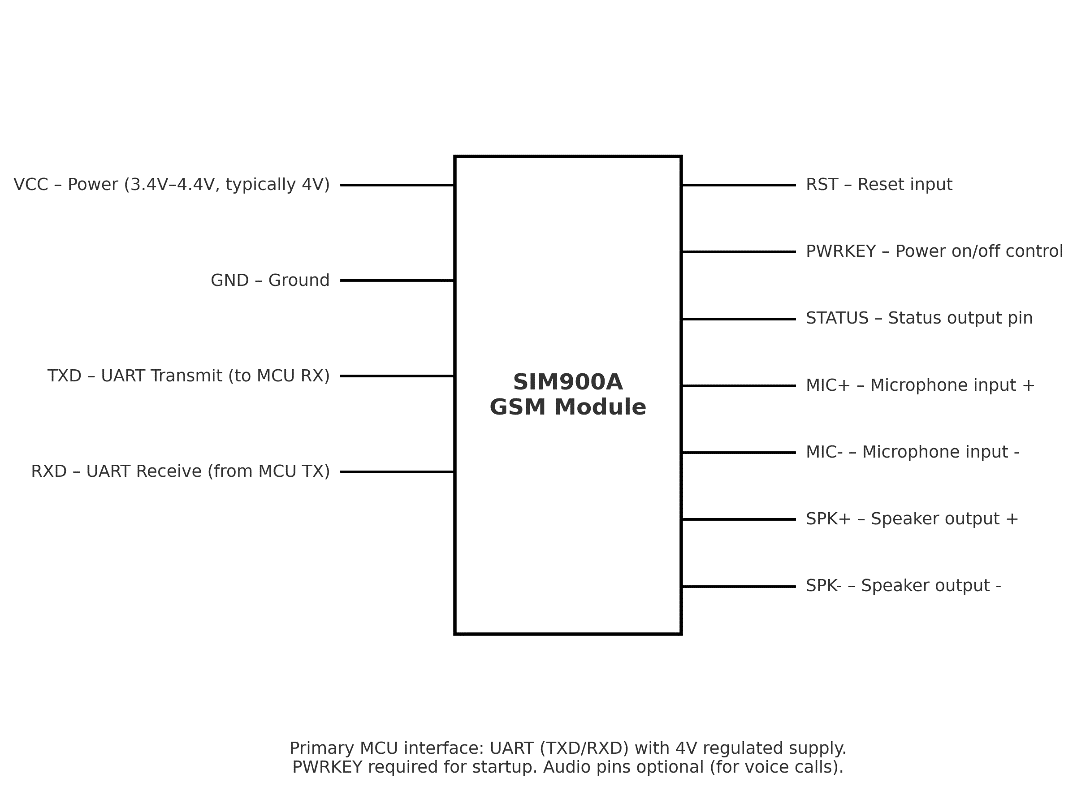
\includegraphics[width=0.8\textwidth]{backmatter/figs/c3.png}
    \caption{SIM900A GSM Module full logical pinout}
    \label{fig:sim900a_pinout}
\end{figure}

\section{NEO M8L GPS Module}

\textbf{Technical Specifications}
\begin{itemize}
    \item Voltage: 3.0–5.0V
    \item Current: ~45 mA
    \item Communication: UART (9600 baud default)
    \item Accuracy: 2.5 m CEP
    \item Cold Start Time: 27 s (average)
\end{itemize}

\textbf{Pin Configuration}

\begin{table}[htbp]
    \centering
    \caption{NEO M8L GPS Module Pin Configuration}
    \label{tab:neo_pins}
    \small
    \begin{tabular}{l l p{5cm} p{5cm}}
        \toprule
        \textbf{Pin No.} & \textbf{Name} & \textbf{Function} & \textbf{Connection} \\
        \midrule
        1 & VCC & Power & 3.3V/5V \\
        2 & GND & Ground & Common GND \\
        3 & TX & Data Out & ESP32 RX16 \\
        4 & RX & Data In & ESP32 TX17 \\
        \bottomrule
    \end{tabular}
\end{table}

\begin{figure}[htbp]
    \centering
    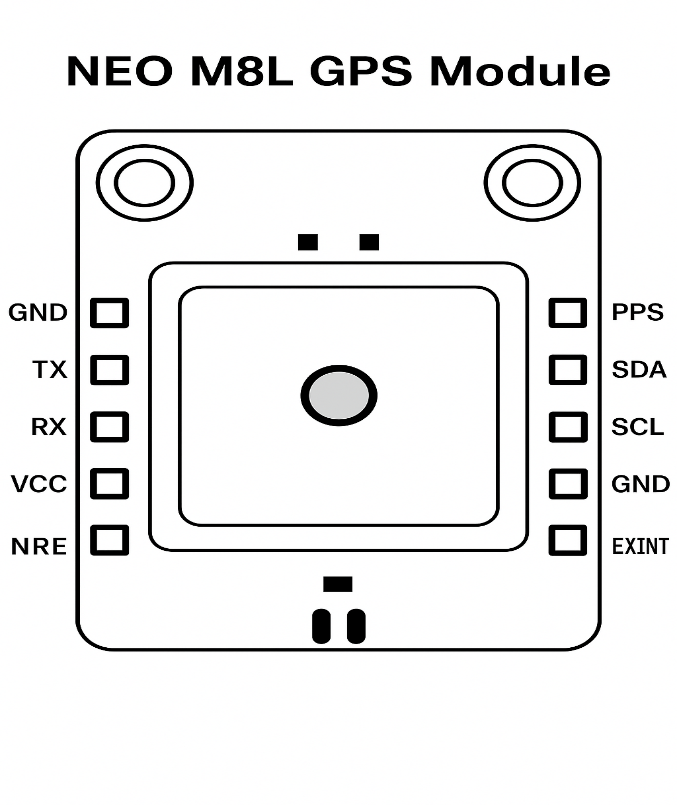
\includegraphics[width=0.8\textwidth]{backmatter/figs/c4.png}
    \caption{NEO M8L GPS Module full logical pinout}
    \label{fig:neo_pinout}
\end{figure}

\section{Micro SD Card Module}

\textbf{Technical Specifications}
\begin{itemize}
    \item Voltage: 3.3V (with onboard regulator for 5V input)
    \item Interface: SPI
    \item Supported: FAT32 file system
\end{itemize}

\textbf{Pin Configuration}

\begin{table}[htbp]
    \centering
    \caption{Micro SD Card Module Pin Configuration}
    \label{tab:sd_pins}
    \small
    \begin{tabular}{l l p{5cm} p{5cm}}
        \toprule
        \textbf{Pin No.} & \textbf{Name} & \textbf{Function} & \textbf{Connection} \\
        \midrule
        1 & VCC & Power & 3.3V/5V \\
        2 & GND & Ground & Common GND \\
        3 & SCK & SPI Clock & ESP32 GPIO5 \\
        4 & MOSI & SPI Data & ESP32 GPIO18 \\
        5 & MISO & SPI Read & ESP32 GPIO19 \\
        6 & CS & Chip Select & ESP32 GPIO4 \\
        \bottomrule
    \end{tabular}
\end{table}

\begin{figure}[htbp]
    \centering
    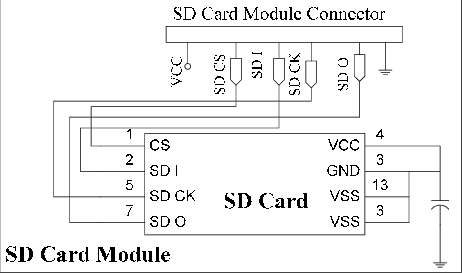
\includegraphics[width=0.8\textwidth]{backmatter/figs/c5.png}
    \caption{Micro SD Card Module (a) and (b) full logical pinout}
    \label{fig:sd_pinout}
\end{figure}

\section{2.8" TFT LCD Display}

\textbf{Technical Specifications}
\begin{itemize}
    \item Voltage: 3.3V
    \item Interface: SPI
    \item Resolution: 240x320 pixels
    \item Display Size: 2.8 inches
\end{itemize}

\textbf{Pin Configuration}

\begin{table}[htbp]
    \centering
    \caption{2.8" TFT LCD Display Pin Configuration}
    \label{tab:lcd_pins}
    \small
    \begin{tabular}{l l p{5cm} p{5cm}}
        \toprule
        \textbf{Pin No.} & \textbf{Name} & \textbf{Function} & \textbf{Connection} \\
        \midrule
        1 & VCC & Power & 3.3V \\
        2 & GND & Ground & Common GND \\
        3 & SCK & SPI Clock & ESP32 GPIO5 \\
        4 & MOSI & SPI Data & ESP32 GPIO18 \\
        5 & MISO & SPI Read & ESP32 GPIO19 \\
        6 & CS & Chip Select & ESP32 GPIO15 \\
        \bottomrule
    \end{tabular}
\end{table}

\begin{figure}[htbp]
    \centering
    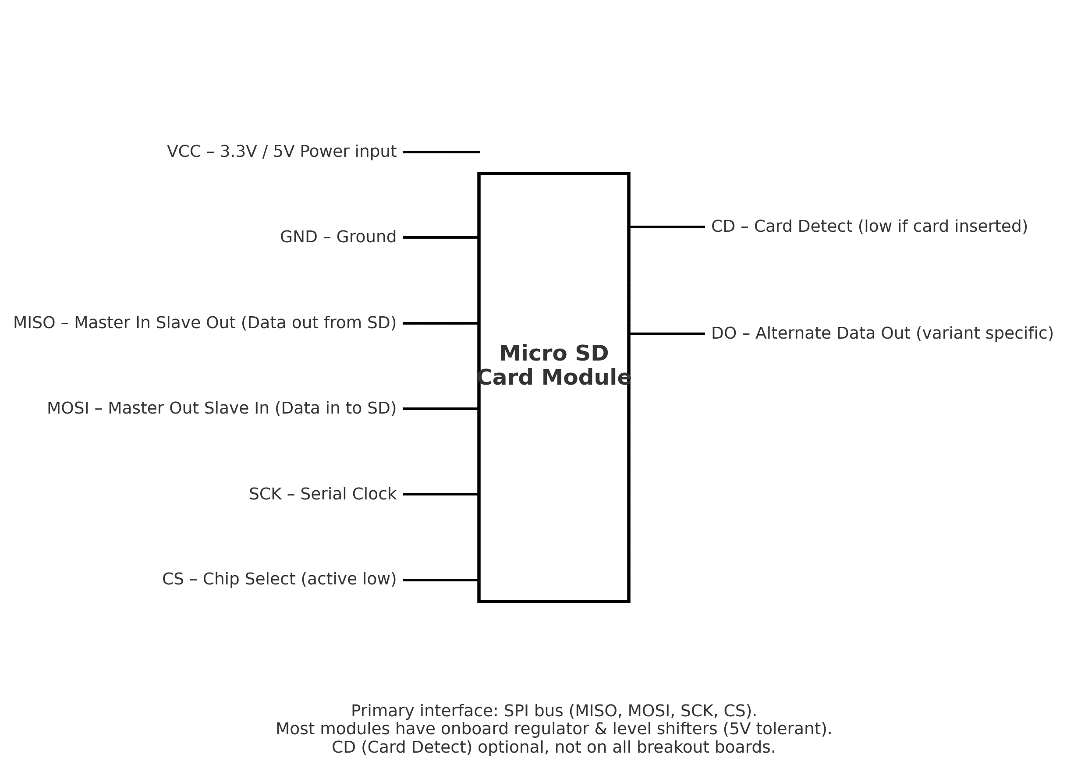
\includegraphics[width=0.8\textwidth]{backmatter/figs/c6.png}
    \caption{2.8" TFT LCD Display full logical pinout}
    \label{fig:lcd_pinout}
\end{figure}

\section{Power Supply and Voltage Regulation}

\textbf{Technical Specifications}
\begin{itemize}
    \item Input: 5V (USB or adapter)
    \item Regulator: AMS1117 (5V → 3.3V)
    \item Max Current: 800mA (per regulator)
\end{itemize}

\begin{figure}[htbp]
    \centering
    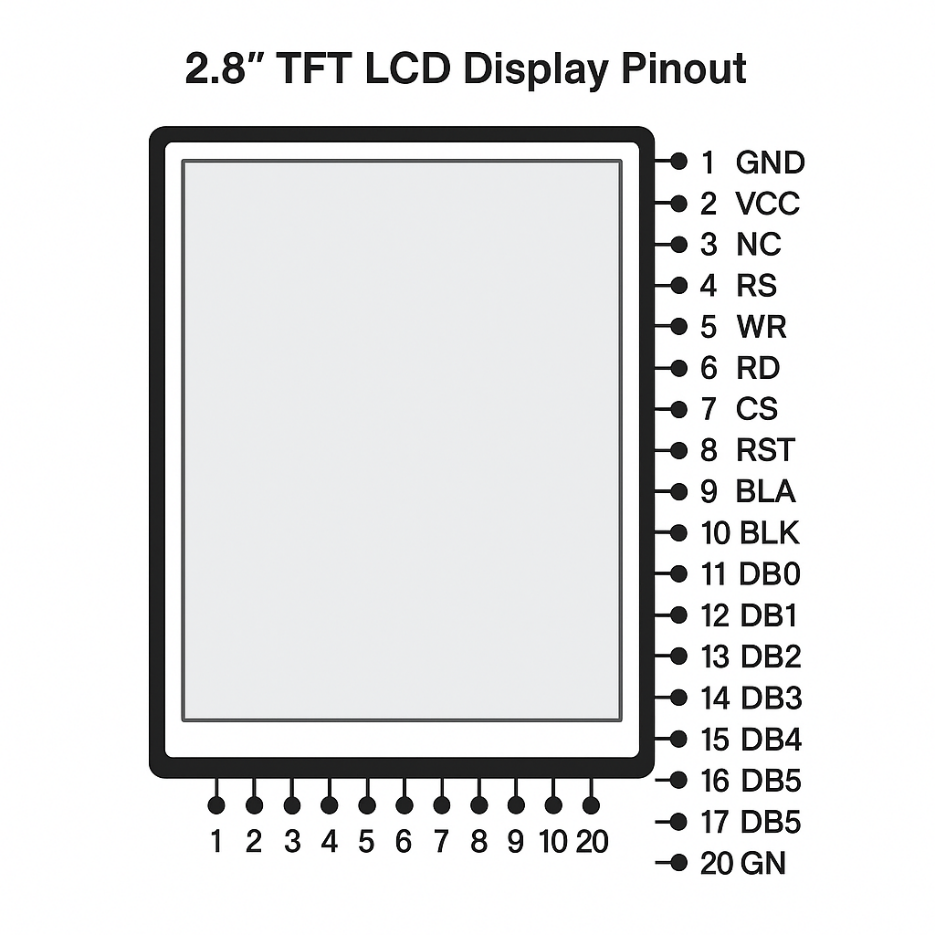
\includegraphics[width=0.8\textwidth]{backmatter/figs/c7.png}
    \caption{Power supply and Regulator Circuit full logical pinout Diagram}
    \label{fig:power_pinout}
\end{figure}

\section{XL6009 Buck Converter}

\textbf{Technical Specifications}
\begin{itemize}
    \item Input Voltage Range: 5 V to 32 V
    \item Output Voltage Range: 1.25 V to 30 V (adjustable)
    \item Maximum Output Current: Up to 3 A (with cooling)
    \item Switching Frequency: Approximately 200 kHz
    \item Efficiency: Up to 94\%
    \item Output Voltage Ripple: Typically, less than 50 mV
    \item Protection Features: Overcurrent and thermal shutdown
    \item Dimensions: Approx. 43 mm × 21 mm × 14 mm
\end{itemize}

\begin{figure}[htbp]
    \centering
    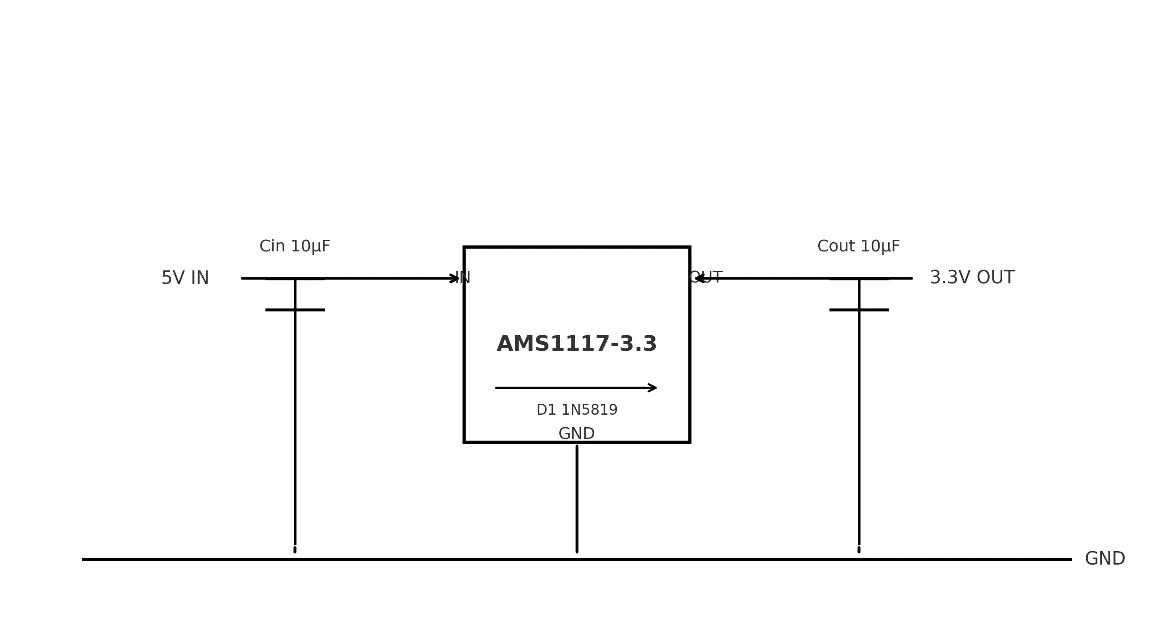
\includegraphics[width=0.8\textwidth]{backmatter/figs/c8.png}  % Or image9.png if needed
    \caption{XL6009 Buck Converter full logical pinout Diagram}
    \label{fig:xl6009_pinout}
\end{figure}

\section{Sir Freed Alvi's Review on Circuit Diagram}

\begin{figure}[htbp]
    \centering
    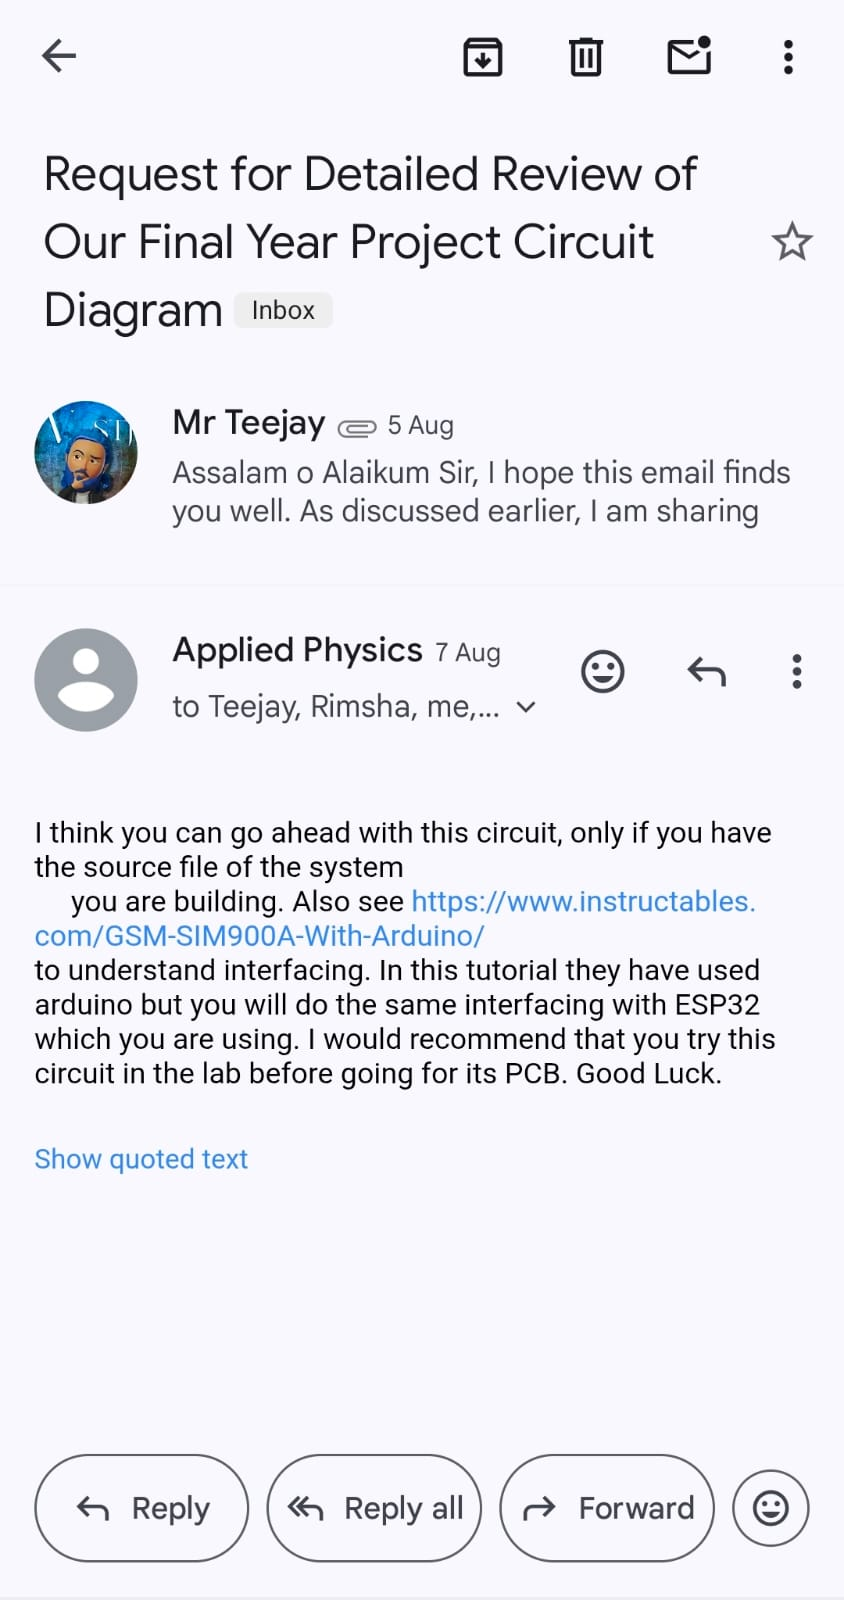
\includegraphics[width=0.8\textwidth]{backmatter/figs/sir fareed' review.png}  % Or image9.png if needed
    \caption{Sir Freed Alvi's Review on Circuit Diagram}
    \label{fig:Sir Freed Alvi's Review on Circuit Diagram}
\end{figure}

% Appendix D: Wokwi Simulation Code and Configuration
\chapter{Wokwi Simulation Code and Configuration}

This appendix presents the complete code and configuration files used in the Wokwi online simulator to prototype and test the vehicle tracking system's core functionality, including LCD display, SD card logging, and simulated GPS data.

\subsection{Main Sketch (sketch.ino)}

\begin{lstlisting}[width=0.8\textwidth][language=C++, caption={Main Arduino Sketch for Wokwi Simulation}, label={lst:wokwi_sketch}, basicstyle=\small\ttfamily, keywordstyle=\color{blue}, stringstyle=\color{red}, commentstyle=\color{green}, numbers=left, numberstyle=\tiny, frame=single]
#include <Adafruit_GFX.h>
#include <Adafruit_ILI9341.h>
#include <SPI.h>
#include <SD.h>

// LCD Pins
#define TFT_CS   15
#define TFT_DC   2
#define TFT_RST  4
Adafruit_ILI9341 tft = Adafruit_ILI9341(TFT_CS, TFT_DC, TFT_RST);

// SD Card Pin
#define SD_CS 5
File dataFile;

// Fake GPS Data
float latitude = 24.8600;
float longitude = 67.0000;

void setup() {
  Serial.begin(115200);

  tft.begin();
  tft.setRotation(1);
  tft.fillScreen(ILI9341_BLACK);
  tft.setTextColor(ILI9341_WHITE);
  tft.setTextSize(2);

  if (!SD.begin(SD_CS)) {
    tft.setCursor(0, 0);
    tft.println("SD Failed!");
    while (1);
  }

  tft.setCursor(0, 0);
  tft.println("System Ready!");

  delay(2000);
}

void loop() {
  // Simulate Dynamic GPS Data
  latitude += 0.0001;    // Fake latitude increment
  longitude += 0.0001;   // Fake longitude increment

  // Display on LCD
  tft.fillScreen(ILI9341_BLACK);
  tft.setCursor(0, 0);
  tft.print("Lat: ");
  tft.println(latitude, 6);

  tft.print("Lon: ");
  tft.println(longitude, 6);

  // Save to SD Card
  dataFile = SD.open("/gpslog.txt", FILE_APPEND);
  if (dataFile) {
    dataFile.print("Lat: ");
    dataFile.print(latitude, 6);
    dataFile.print(", Lon: ");
    dataFile.println(longitude, 6);
    dataFile.close();
    Serial.println("Data saved.");
  } else {
    Serial.println("File write error.");
  }

  delay(2000);  // 2 seconds delay (simulate tracking interval)
}
\end{lstlisting}

\subsection{Diagram Configuration (diagram.json)}
\begin{adjustbox}{width=\textwidth}
\begin{lstlisting}
[language=JSON, caption={Wokwi Diagram Configuration JSON}, label={lst:wokwi_diagram}, basicstyle=\small\ttfamily, frame=single]
{
  "version": 1,
  "author": "Saman Aslam",
  "editor": "wokwi",
  "parts": [
    { "type": "board-esp32-devkit-c-v4", "id": "esp", "top": 0, "left": 0, "attrs": {} },
    { "type": "wokwi-microsd-card", "id": "sd1", "top": -86.17, "left": -124.73, "attrs": {} },
    { "type": "wokwi-ili9341", "id": "lcd1", "top": -37.6, "left": -355.5, "attrs": {} },
    { "type": "chip-gps-module", "id": "chip1", "top": -56.58, "left": 235.2, "attrs": {} },
    { "type": "chip-nfc-reader-em-18", "id": "chip2", "top": 49.02, "left": 235.2, "attrs": {} },
    {
      "type": "chip-gsm-module-sim900a",
      "id": "chip3",
      "top": 173.82,
      "left": 235.2,
      "attrs": {}
    }
  ],
  "connections": [
    [ "esp:TX", "$serialMonitor:RX", "", [] ],
    [ "esp:RX", "$serialMonitor:TX", "", [] ],
    [ "lcd1:VCC", "esp:5V", "red", [ "v9.6", "h297.6", "v-57.6" ] ],
    [ "lcd1:GND", "esp:GND.2", "black", [ "v19.2", "h412.8", "v-240" ] ],
    [ "lcd1:CS", "esp:15", "green", [ "v28.8", "h412.8", "v-48" ] ],
    [ "lcd1:RST", "esp:4", "green", [ "v38.4", "h412.8", "v-144" ] ],
    [ "lcd1:D/C", "esp:2", "green", [ "v48", "h412.8", "v-134.4" ] ],
    [ "lcd1:MOSI", "esp:23", "green", [ "v57.6", "h412.79", "v-9.6" ] ],
    [ "lcd1:SCK", "esp:18", "green", [ "v67.2", "h412.79", "v-9.6" ] ],
    [ "lcd1:LED", "esp:5V", "green", [ "v76.8", "h211.19", "v-124.8" ] ],
    [ "sd1:CS", "esp:5", "green", [ "h172.8", "v134.46" ] ],
    [ "sd1:SCK", "esp:18", "green", [ "h182.4", "v153.59" ] ],
    [ "sd1:DO", "esp:19", "green", [ "h192", "v0.11" ] ],
    [ "sd1:DI", "esp:23", "green", [ "h201.6", "v-0.09" ] ],
    [ "sd1:VCC", "esp:5V", "red", [ "h28.8", "v0.14" ] ],
    [ "sd1:GND", "esp:GND.2", "black", [ "h211.2", "v0.11" ] ],
    [ "chip1:OUT", "esp:TX", "green", [ "h21.01", "v48", "h-163.2", "v9.6" ] ],
    [ "chip2:OUT", "esp:TX", "green", [ "h21.01", "v38.4", "h-192", "v-38.4", "h-9.6" ] ],
    [ "chip3:OUT", "esp:TX", "green", [ "h21.01", "v-38.4", "h-172.8", "v-86.4" ] ],
    [ "esp:RX", "chip1:IN", "green", [ "h120.04", "v-48", "h134.4", "v-9.6" ] ],
    [ "esp:RX", "chip2:IN", "green", [ "h110.44", "v38.4", "h144", "v-38.4" ] ],
    [ "esp:RX", "chip3:IN", "green", [ "h81.64", "v153.6", "h182.4", "v-28.8" ] ]
  ],
  "dependencies": {}
}
\end{lstlisting}
\end{adjustbox}

\subsection{Custom Chip Definitions}

The simulation uses custom chips for GPS, NFC, and GSM modules. Their configurations and basic C implementations are provided below.

\textbf{gps-module.chip.json, nfc-reader-em-18.chip.json, and gsm-module-sim900a.chip.json} (similar structure):

\begin{lstlisting}
[language=JSON, caption={Example Custom Chip JSON 
(gps-module.chip.json)}
, label={lst:custom_chip_json}]
{
  "name": "gps-module",
  "author": "Saman Aslam",
  "pins": [
    "VCC",
    "GND",
    "IN",
    "OUT"
  ],
  "controls": []
}
\end{lstlisting}

\textbf{Custom Chip C Code} (identical placeholder for all three modules):

\begin{lstlisting}[language=C, caption={Custom Chip C Implementation (e.g., gps-module.chip.c)}, label={lst:custom_chip_c}]
#include "wokwi-api.h"
#include <stdio.h>
#include <stdlib.h>

typedef struct {
  // TODO: Put your chip variables here
} chip_state_t;

void chip_init() {
  chip_state_t *chip = malloc(sizeof(chip_state_t));

  printf("Hello from custom chip!\n");
}
\end{lstlisting}

\subsection{Required Libraries}

\begin{itemize}
    \item Adafruit GFX Library
    \item Adafruit ILI9341 Library
\end{itemize}

\subsection{Current Implemented Sketch}

\begin{lstlisting}[language=C++, caption={Main Arduino Sketch of current Implementation}, label={lst:wokwi_sketch}, basicstyle=\small\ttfamily, breaklines=true, keywordstyle=\color{blue}, stringstyle=\color{red}, commentstyle=\color{green}, numbers=left, numberstyle=\tiny, frame=single]
#include <WiFi.h>
#include <WiFiClientSecure.h>  //  Changed from WiFiClient
#include <PubSubClient.h>
#include <Adafruit_GFX.h>
#include <Adafruit_ST7789.h>
#include <Wire.h>
#include <Adafruit_PN532.h>
#include <SPI.h>
#include "time.h"

// ----------------- Wi-Fi + MQTT -----------------
const char* ssid = "taha";
const char* password = "taha1234";

// HiveMQ Cloud Configuration
const char* mqtt_server = "84837c1224714acc85e9e0935388600d.s1.
eu.hivemq.cloud";
const int mqtt_port = 8883; // Secure MQTT port
const char* mqtt_user = "taha_user";
const char* mqtt_pass = "Strongpassword123";

// NTP server
const char* ntpServer = "pool.ntp.org";
const long gmtOffset_sec = 5 * 3600;
const int daylightOffset_sec = 0;

WiFiClientSecure espClient;  // ✅ Changed to WiFiClientSecure
PubSubClient client(espClient);

// Device + vehicle identity
String DEVICE_ID = "DVC001";
String VEHICLE_NUM = "V001";

// ----------------- Display setup -----------------
#define TFT_CS  9
#define TFT_DC  8
#define TFT_RST 7

Adafruit_ST7789 tft = Adafruit_ST7789(TFT_CS, TFT_DC, TFT_RST);

// ----------------- NFC setup -----------------
#define SDA_PIN      21
#define SCL_PIN      47
#define PN532_IRQ     2
#define PN532_RESET   4

Adafruit_PN532 nfc(PN532_IRQ, PN532_RESET, &Wire);

// ----------------- State variables -----------------
bool waitingForDispatchTap = false;
bool waitingForResolveTap = false;
bool allowNFCTap = false;

String activeFaultId = "";
String activeFaultDetails = "";

unsigned long faultDisplayStart = 0;

// ----------------- Time -----------------
void setupTime() {
  configTime(gmtOffset_sec, daylightOffset_sec, ntpServer);
  
  // Wait for time to sync
  Serial.print("⏳ Syncing time");
  int attempts = 0;
  while (getCurrentTimeString() == "--:--:--" && attempts < 30) {
    delay(500);
    Serial.print(".");
    attempts++;
  }
  Serial.println();
  
  if (getCurrentTimeString() != "--:--:--") {
    Serial.println("✅ Time synced: " + getCurrentTimeString());
  } else {
    Serial.println("⚠️ Time sync failed, but continuing...");
  }
}

String getCurrentTimeString() {
  struct tm timeinfo;
  if (!getLocalTime(&timeinfo)) return "--:--:--";
  char buffer[16];
  strftime(buffer, sizeof(buffer), "%H:%M:%S", &timeinfo);
  return String(buffer);
}

// ----------------- UI -----------------
void drawBaseUI() {
  tft.fillScreen(ST77XX_BLACK);
  tft.drawLine(0, 40, 240, 40, ST77XX_WHITE);
  tft.drawLine(0, 280, 240, 280, ST77XX_WHITE);

  tft.setTextSize(1);
  tft.setTextColor(ST77XX_WHITE);
  tft.setCursor(5, 10);
  tft.print("Time: --:--:--");

  tft.setCursor(180, 10);
  tft.print("Wi-Fi: ...");

  tft.setTextSize(2);
  tft.setCursor(60, 130);
  tft.print("On Hold...");

  tft.setTextSize(2);
  tft.setCursor(60, 285);
  tft.print("TappTrack");
}

void updateTopBar() {
  tft.fillRect(0, 0, 240, 40, ST77XX_BLACK);
  tft.setTextSize(1);
  tft.setTextColor(ST77XX_WHITE);
  tft.setCursor(5, 10);
  tft.print("Time: " + getCurrentTimeString());

  tft.setCursor(180, 10);
  tft.print("Wi-Fi:");
  if (WiFi.status() == WL_CONNECTED)
    tft.print(" OK");
  else
    tft.print(" ...");
}

void showDispatchBox(String msg) {
  tft.fillRect(20, 80, 200, 160, ST77XX_BLUE);
  tft.setTextColor(ST77XX_WHITE);
  tft.setTextSize(2);
  tft.setCursor(30, 140);
  tft.print("Dispatch!");
  tft.setTextSize(1);
  tft.setCursor(30, 180);
  tft.print("Tap NFC to confirm");
}

void showFaultDetails(String details) {
  tft.fillRect(20, 80, 200, 160, ST77XX_GREEN);
  tft.setTextColor(ST77XX_BLACK);
  tft.setTextSize(1);

  int y = 90;
  int x = 25;
  String word = "";
  for (int i = 0; i < details.length(); i++) {
    char c = details[i];
    if (c == ' ' || i == details.length() - 1) {
      if (i == details.length() - 1) word += c;
      tft.setCursor(x, y);
      tft.print(word);
      y += 15;
      word = "";
    } else word += c;
  }
}

void showTapInstruction() {
  tft.setTextSize(1);
  tft.setTextColor(ST77XX_BLACK);
  tft.setCursor(35, 210);
  tft.print("NFC enabled - Tap to mark as resolved");
}

// ----------------- MQTT -----------------
void callback(char* topic, byte* payload, unsigned int length) {
  String msg;
  for (int i = 0; i < length; i++) msg += (char)payload[i];

  Serial.println("�� Received message:");
  Serial.println("Topic: " + String(topic));
  Serial.println("Payload: " + msg);

  String expectedTopic = "device/" + DEVICE_ID + "/dispatch";
  if (String(topic) == expectedTopic) {
    int fidStart = msg.indexOf("\"fault_id\":\"");
    int detailsStart = msg.indexOf("\"fault_details\":\"");

    if (fidStart != -1) {
      fidStart += 12;
      int fidEnd = msg.indexOf("\"", fidStart);
      activeFaultId = msg.substring(fidStart, fidEnd);
    } else activeFaultId = "unknown";

    if (detailsStart != -1) {
      detailsStart += 17;
      int detailsEnd = msg.indexOf("\"", detailsStart);
      activeFaultDetails = msg.substring(detailsStart, 
      detailsEnd);
    } else activeFaultDetails = "No details";

    Serial.println("Fault ID: " + activeFaultId);
    Serial.println("Details: " + activeFaultDetails);

    showDispatchBox("Dispatch Received! Tap NFC to Confirm");
    waitingForDispatchTap = true;
  }
}

// ----------------- Wi-Fi + MQTT -----------------
void setup_wifi() {
  Serial.println("�� Connecting to WiFi: " + String(ssid));
  WiFi.begin(ssid, password);
  
  int attempts = 0;
  while (WiFi.status() != WL_CONNECTED && attempts < 40) {
    delay(500);
    Serial.print(".");
    attempts++;
  }
  
  Serial.println();
  if (WiFi.status() == WL_CONNECTED) {
    Serial.println("✅ WiFi Connected!");
    Serial.print("IP Address: ");
    Serial.println(WiFi.localIP());
  } else {
    Serial.println("❌ WiFi Connection Failed!");
  }
}

void reconnect() {
  while (!client.connected()) {
    Serial.print("�� Connecting to MQTT broker: ");
    Serial.println(mqtt_server);
    
    // Generate unique client ID
    String clientId = "ESP32_" + DEVICE_ID + "_" + String(random
    (0xffff), HEX);
    
    // ✅ Added username and password
    if (client.connect(clientId.c_str(), mqtt_user, mqtt_pass)) {
      Serial.println("✅ MQTT Connected!");
      
      // Subscribe to dispatch topic
      String topic = "device/" + DEVICE_ID + "/dispatch";
      if (client.subscribe(topic.c_str())) {
        Serial.println("�� Subscribed to: " + topic);
      } else {
        Serial.println("❌ Subscription failed!");
      }
    } else {
      Serial.print("❌ MQTT Connection Failed! Error code: ");
      Serial.println(client.state());
      Serial.println("Retrying in 5 seconds...");
      delay(5000);
    }
  }
}

// ----------------- Setup -----------------
void setup() {
  Serial.begin(115200);
  delay(1000);
  Serial.println("\n\n�� TappTrack ESP32 Starting...");
  Serial.println("================================");
  
  // Initialize Display
  Serial.println("��️  Initializing display...");
  Wire.begin(SDA_PIN, SCL_PIN);
  tft.init(240, 320);
  drawBaseUI();
  Serial.println("✅ Display ready");

  // Initialize NFC
  Serial.println("�� Initializing NFC reader...");
  nfc.begin();
  uint32_t versiondata = nfc.getFirmwareVersion();
  if (!versiondata) {
    Serial.println("❌ PN532 not found!");
    while (1) delay(100);
  }
  Serial.println("✅ PN532 Found!");
  nfc.SAMConfig();

  // Connect to WiFi
  setup_wifi();
  
  // Setup secure MQTT connection
  Serial.println("�� Setting up secure MQTT...");
  espClient.setInsecure();  // Skip certificate verification
  client.setServer(mqtt_server, mqtt_port);  
  // ✅ Using mqtt_port (8883)
  client.setCallback(callback);
  client.setKeepAlive(60);
  client.setSocketTimeout(30);
  Serial.println("✅ MQTT client configured");
  
  // Setup time (required for TLS)
  setupTime();
  
  // Initial MQTT connection
  reconnect();
  
  Serial.println("================================");
  Serial.println("✅ Setup Complete! Device: " + DEVICE_ID);
  Serial.println("✅ Vehicle: " + VEHICLE_NUM);
  Serial.println("✅ Waiting for dispatch...\n");
}

// ----------------- Loop -----------------
void loop() {
  updateTopBar();
  
  // Maintain MQTT connection
  if (!client.connected()) {
    Serial.println("⚠️ MQTT disconnected, reconnecting...");
    reconnect();
  }
  client.loop();

  uint8_t uid[7];
  uint8_t uidLength;

  // --- Step 1: Wait for NFC to confirm dispatch ---
  if (waitingForDispatchTap) {
    if (nfc.readPassiveTargetID(PN532_MIFARE_ISO14443A, uid, 
    &uidLength)) {
      Serial.println("✅ Dispatch confirmed via NFC!");
      waitingForDispatchTap = false;

      // Notify MQTT
      String payload = "{\"confirmed\":true,\"device_id\":\""
      + DEVICE_ID +
                       "\",\"vehicle_number\":\"" + VEHICLE_NUM 
                       +
                       "\",\"fault_id\":\"" + activeFaultId + "\"}";
      
      if (client.publish(("vehicle/" + VEHICLE_NUM + 
      "/confirmation").c_str(), payload.c_str())) {
        Serial.println("�� Confirmation sent successfully");
      } else {
        Serial.println("❌ Failed to send confirmation");
      }

      // Show fault details now
      showFaultDetails(activeFaultDetails);
      faultDisplayStart = millis();
      waitingForResolveTap = true;
      allowNFCTap = false;
    }
  }

  // --- Step 2: Show fault details & enable NFC after 10s ---
  if (waitingForResolveTap) {
    if (!allowNFCTap && millis() - faultDisplayStart >= 10000) {
      allowNFCTap = true;
      showTapInstruction();
      Serial.println("�� NFC tap enabled for resolution");
    }

    // --- Step 3: Wait for NFC tap to mark resolved ---
    if (allowNFCTap) {
      if (nfc.readPassiveTargetID(PN532_MIFARE_ISO14443A, 
      uid, &uidLength)) {
        Serial.println("✅ NFC Tap detected, marking as
        resolved...");
        waitingForResolveTap = false;
        allowNFCTap = false;

        String payload = "{\"resolved\":true,"
                         "\"device_id\":\"" + DEVICE_ID +
                         "\",\"vehicle_number\":\"" + 
                         VEHICLE_NUM +
                         "\",\"fault_id\":\"" + activeFaultId
                         + "\"}";
        
        if (client.publish(("vehicle/" + VEHICLE_NUM +
        "/resolved").c_str(), payload.c_str())) {
          Serial.println("�� Resolution sent successfully");
        } else {
          Serial.println("❌ Failed to send resolution");
        }

        delay(1000);
        drawBaseUI(); // back to On Hold
        activeFaultId = "";
        activeFaultDetails = "";
        Serial.println("�� Back to idle state\n");
      }
    }
  }

  delay(100);
}
\end{lstlisting}
% Appendix E: Hardware Components Purchase Receipts
\chapter{Hardware Components Purchase Receipts}

This appendix includes scanned copies/receipts (pay slips) of the purchases for the key hardware components used in the project prototype. These documents verify the acquisition and associated costs of the components.

\begin{figure}[htbp]
    \centering
    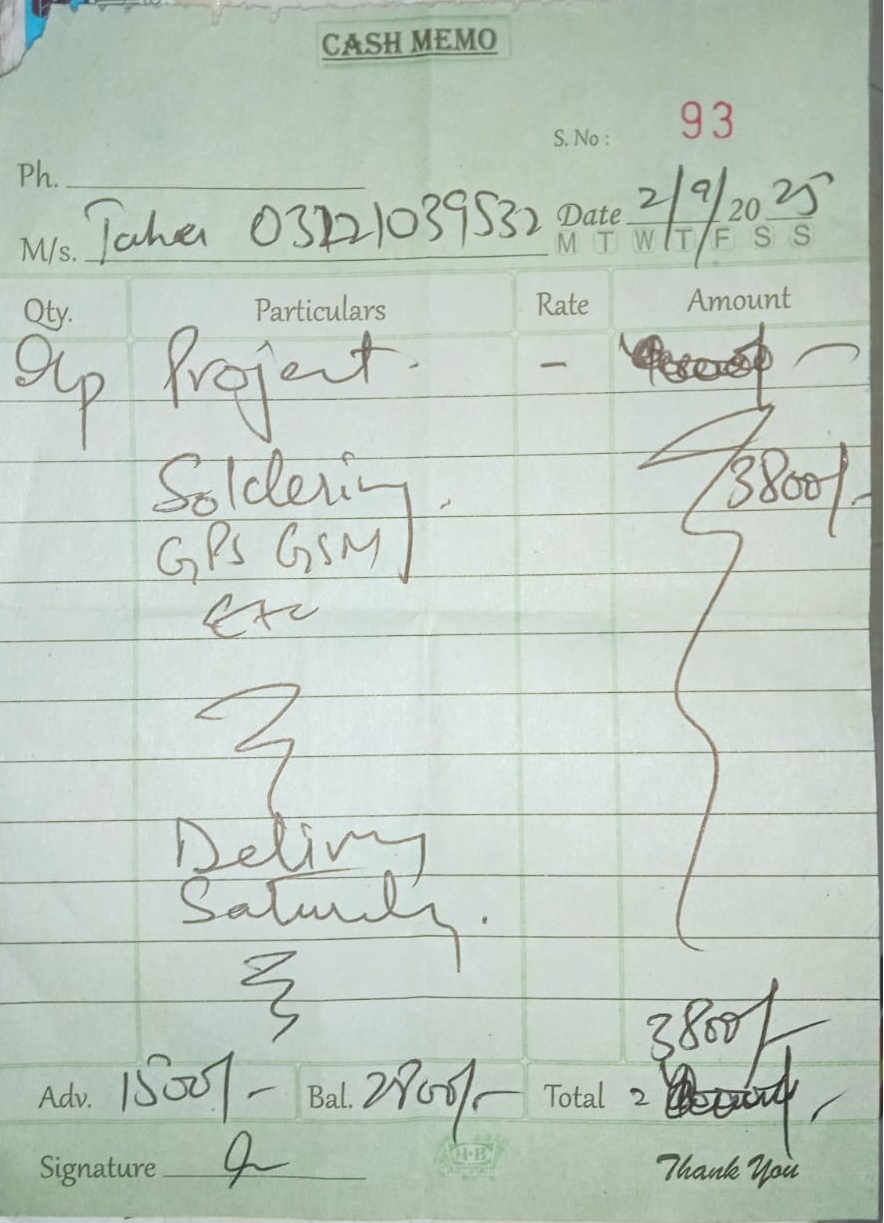
\includegraphics[width=0.9\textwidth]{backmatter/figs/E1.jpg}
    \caption{Purchase Receipt 1 (e.g., ESP32-S3 or related component)}
    \label{fig:receipt1}
\end{figure}

\begin{figure}[htbp]
    \centering
    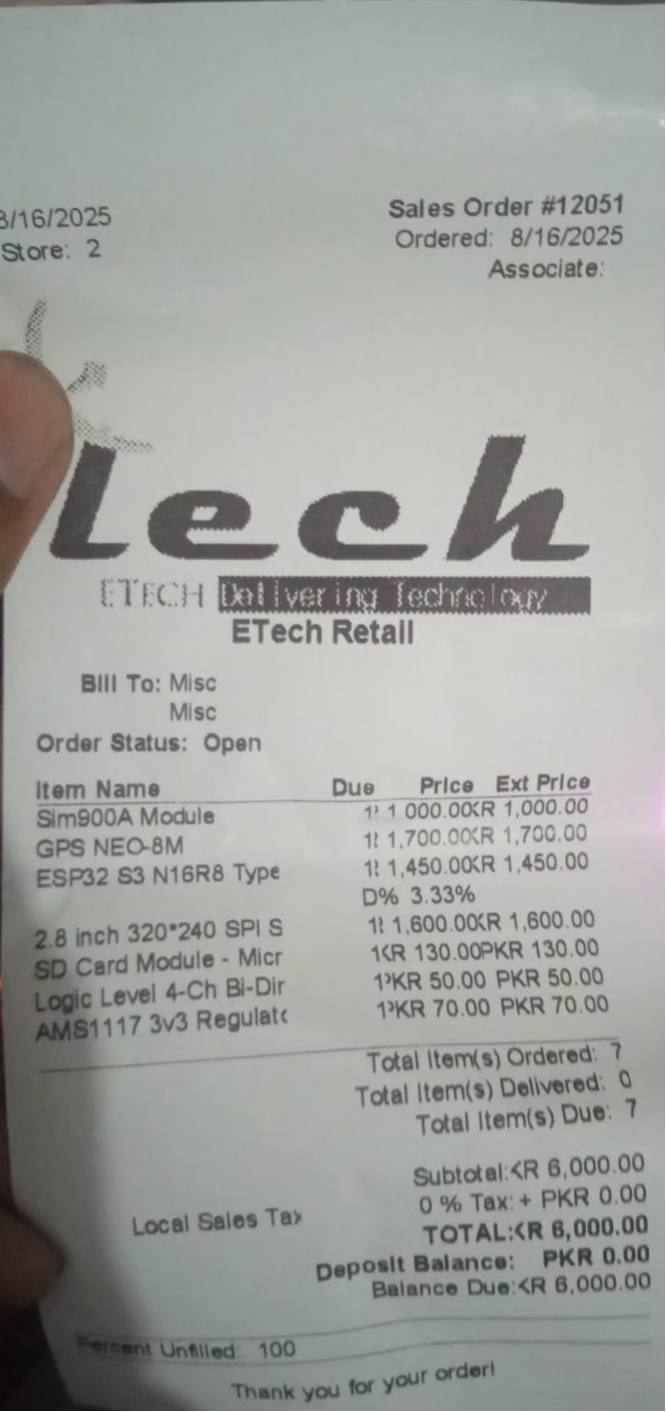
\includegraphics[width=0.9\textwidth]{backmatter/figs/E2.png}
    \caption{Purchase Receipt 2 (e.g., PN532 NFC Reader or related component)}
    \label{fig:receipt2}
\end{figure}

\begin{figure}[htbp]
    \centering
    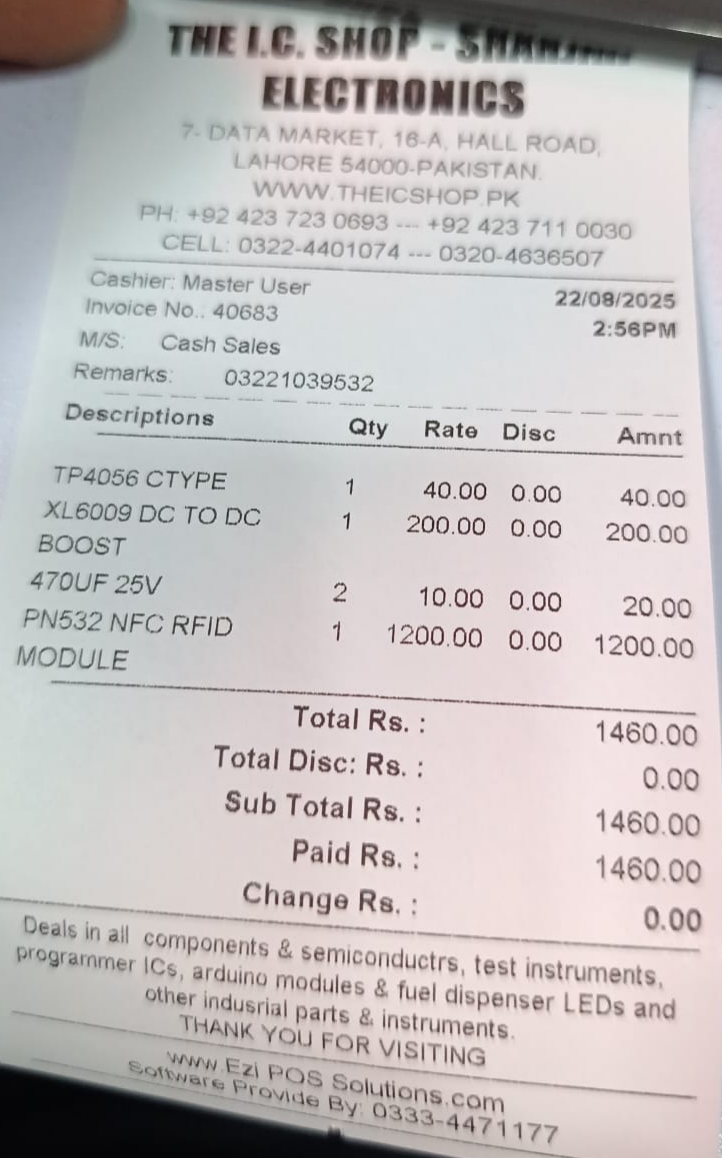
\includegraphics[width=0.9\textwidth]{backmatter/figs/E3.png}
    \caption{Purchase Receipt 3 (e.g., SIM900A GSM Module or related component)}
    \label{fig:receipt3}
\end{figure}

\begin{figure}[htbp]
    \centering
    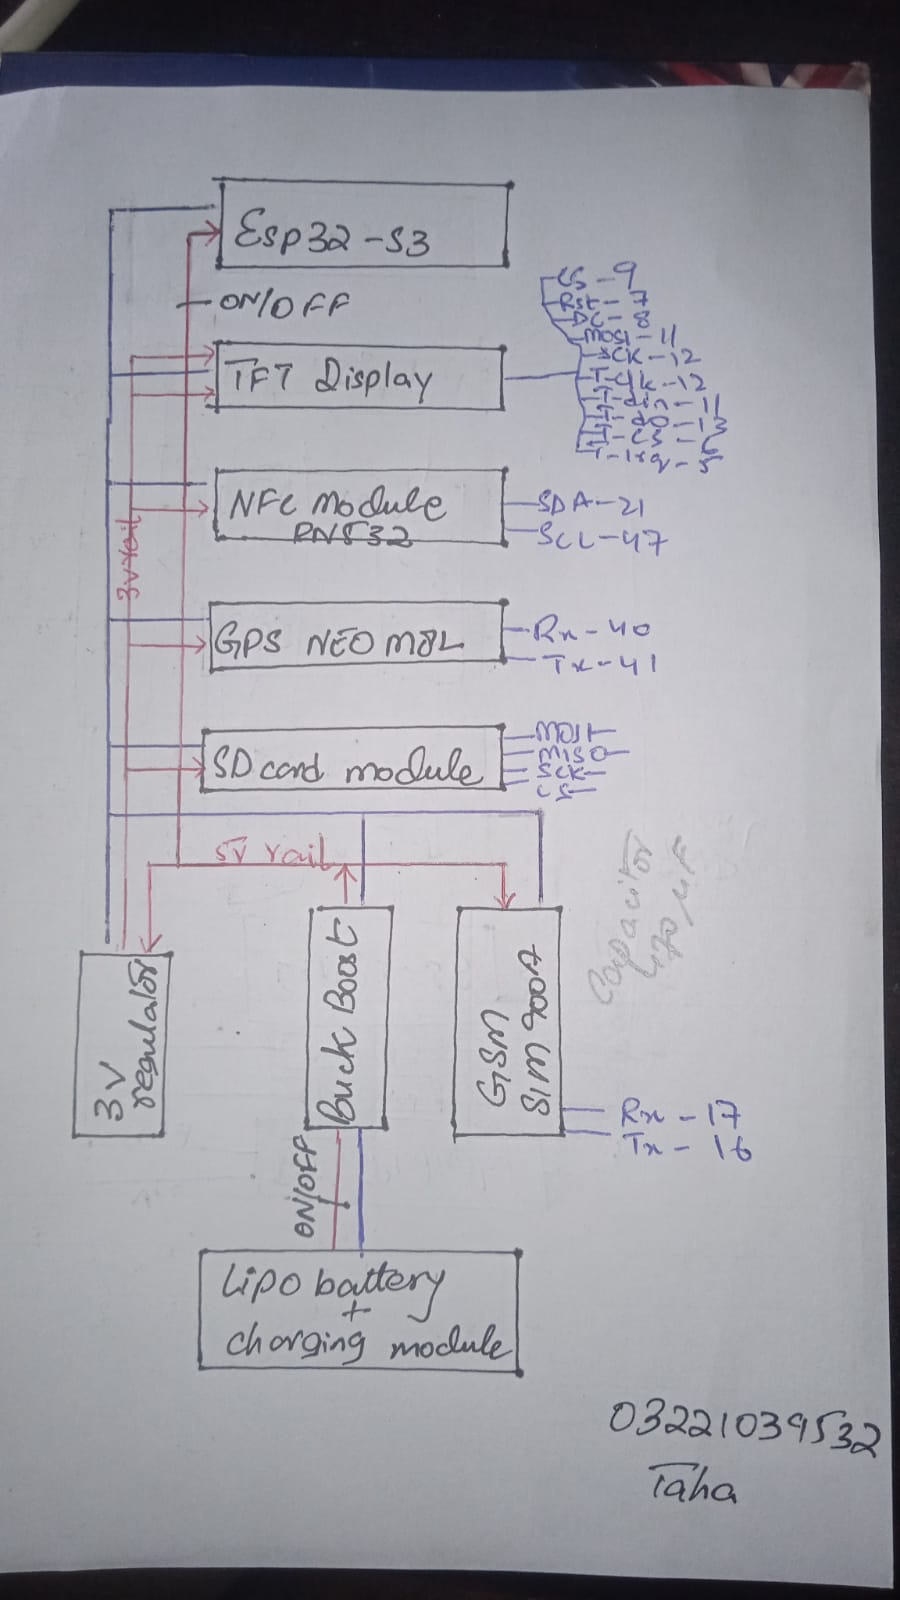
\includegraphics[width=0.9\textwidth]{backmatter/figs/E4.png}
    \caption{Purchase Receipt 4 (e.g., NEO M8L GPS Module or related component)}
    \label{fig:receipt4}
\end{figure}

\begin{figure}[htbp]
    \centering
    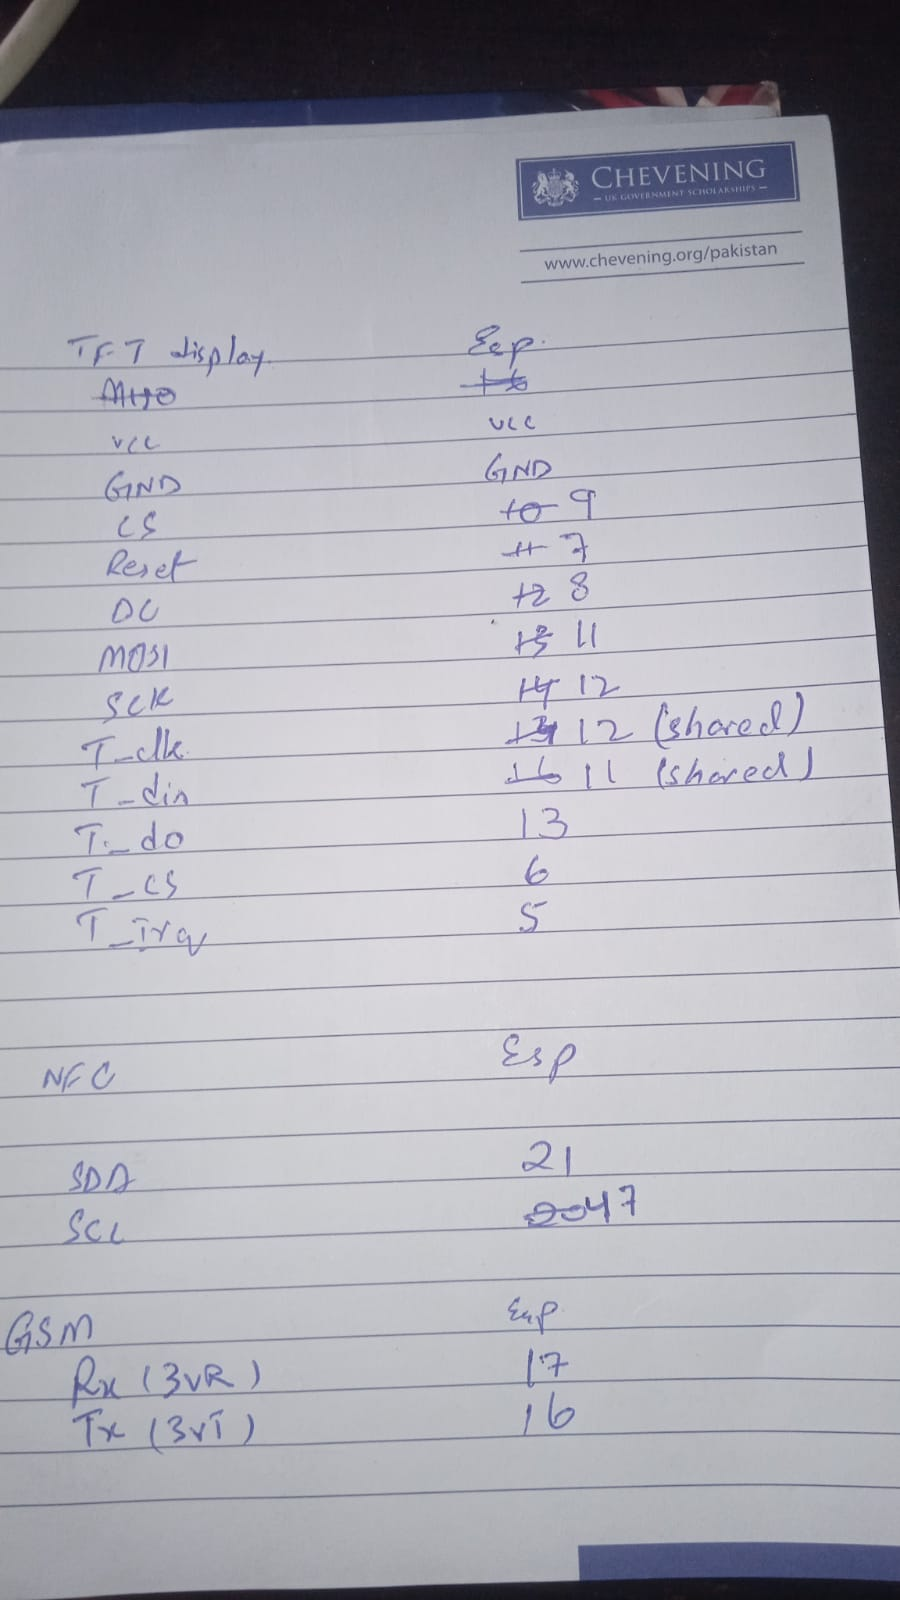
\includegraphics[width=0.9\textwidth]{backmatter/figs/E5.png}
    \caption{Purchase Receipt 5 (e.g., Additional components such as TFT LCD, SD Card Module, or power supplies)}
    \label{fig:receipt5}
\end{figure}


% Appendix F: AI Dispatch Model Features, Training, and API Integration
\chapter{AI Dispatch Model Features, Training, and API Integration}

This appendix details the machine learning model used for intelligent vehicle dispatching, including input features, rule-based target calculation, API endpoints, backend integration, synthetic training data generation, and performance metrics.

\section{Model Features (6 Features)}

\begin{enumerate}
    \item \textbf{distance\_m (float)}
    \begin{itemize}
        \item Description: Distance from vehicle to fault location in meters
        \item Range: 0 to $\sim$50,000+ meters
        \item Calculation: OSRM route distance (with Haversine fallback)
        \item Impact: Lower distance = higher score
    \end{itemize}
    
    \item \textbf{distance\_cat (int)}
    \begin{itemize}
        \item Description: Distance category for categorical encoding
        \item Values: 0: $<$ 1,000 meters; 1: 1,000–5,000 meters; 2: $\geq$ 5,000 meters
        \item Calculation: Categorized from distance\_m
    \end{itemize}
    
    \item \textbf{past\_perf (float)}
    \begin{itemize}
        \item Description: Historical performance score
        \item Range: 1.0 to 10.0
        \item Calculation: (performance\_ratio $\times$ 9) + 1 (where performance ratio: 0.0 worst to 1.0 best)
        \item Source: Historical fault resolution success rate
    \end{itemize}
    
    \item \textbf{fault\_history (int)}
    \begin{itemize}
        \item Description: Count of similar fault types handled by vehicle
        \item Range: 0 to unlimited
        \item Calculation: Count of resolved faults for vehicle
        \item Impact: Higher count = more experience = higher score
    \end{itemize}
    
    \item \textbf{fatigue\_h (float)}
    \begin{itemize}
        \item Description: Crew fatigue in hours
        \item Range: 0.0 to 24.0 hours
        \item Calculation: min(fatigue\_count $\times$ 2, 24)
        \item Fatigue count: Number of faults handled today
        \item Impact: Lower fatigue = higher score
    \end{itemize}
    
    \item \textbf{fault\_severity (int)}
    \begin{itemize}
        \item Description: Fault severity level
        \item Values: 1: Low priority; 2: Medium priority; 3: High priority
        \item Mapping: "Low" $\to$ 1; "Medium" $\to$ 2; "High" $\to$ 3
        \item Source: Fault category field
    \end{itemize}
\end{enumerate}

\section{Model Training: Rule-Based Score Calculation (Training Target)}

The synthetic training targets are generated using the following weighted rule-based score:

\begin{align*}
\text{rule\_score} &= 0.45 \times \text{distance\_score} & \text{\# Distance (inverse normalized)} \\
&+ 0.25 \times \text{fault\_history\_score} & \text{\# Fault history (normalized)} \\
&+ 0.15 \times \text{fatigue\_score} & \text{\# Fatigue (inverse normalized)} \\
&+ 0.05 \times \text{severity\_score} & \text{\# Severity (normalized)} \\
&+ 0.10 \times \text{performance\_score} & \text{\# Performance (normalized)}
\end{align*}

Normalized to 0–100 scale.

\section{API Endpoints}

\subsection{Health Check}

Example Response:
\begin{lstlisting}[language=JSON, caption={Health Check Endpoint Response}, label={lst:health_check}]
{
  "status": "healthy",
  "model_loaded": true,
  "model_features": 6,
  "error": null
}
\end{lstlisting}

\subsection{Model Information}

Example Response:
\begin{lstlisting}[language=JSON, caption={Model Information Endpoint Response}, label={lst:model_info}]
{
  "loaded": true,
  "features": [
    "distance_m",
    "distance_cat",
    "past_perf",
    "fault_history",
    "fatigue_h",
    "fault_severity"
  ],
  "n_features": 6,
  "model_type": "RandomForestRegressor",
  "model_info": {
    "n_estimators": 200,
    "random_seed": 42,
    "training_samples": 2400,
    "test_samples": 600,
    "mae": 2.345,
    "r2": 0.987
  },
  "model_path": "models/dispatch_ml_model.pkl",
  "error": null
}
\end{lstlisting}

\subsection{Predict Best Vehicle}

Example Request Body:
\begin{lstlisting}[language=JSON, caption={Predict Endpoint Request Example}, label={lst:predict_request}]
{
  "candidates": [
    {
      "distance_m": 1250.5,
      "distance_cat": 1,
      "past_perf": 8.2,
      "fault_history": 2,
      "fatigue_h": 4.0,
      "fault_severity": 3
    },
    {
      "distance_m": 3500.0,
      "distance_cat": 1,
      "past_perf": 6.5,
      "fault_history": 0,
      "fatigue_h": 8.0,
      "fault_severity": 3
    }
  ]
}
\end{lstlisting}

Example Response:
\begin{lstlisting}[language=JSON, caption={Predict Endpoint Response Example}, label={lst:predict_response}]
{
  "best_index": 0,
  "scores": [85.3, 72.1],
  "predictions": [ ... ]  % Full array as in document
}
\end{lstlisting}

\subsection{Train Model}

Example Request and Response details as provided in the project documentation.

\section{Integration with Backend and Feature Extraction}

The backend integrates with the ML service via environment variables and batch-optimized feature extraction (e.g., concurrent distance calculations, batch database queries for performance and fatigue).

Example extracted feature object:
\begin{lstlisting}[language=JSON, caption={Example Extracted Feature Object}, label={lst:feature_object}]
{
  "distance_m": 1250,
  "distance_cat": 1,
  "past_perf": 8.2,
  "fault_history": 5,
  "fatigue_h": 4.0,
  "fault_severity": 3
}
\end{lstlisting}

\chapter{Project Resources}
\label{app:project-resources}
The complete source code, documentation, and related resources for the AI Powered Fleet Management and Visibility System are available online:
\begin{itemize}
    \item \textbf{GitHub Repository:} 
    
    \url{https://github.com/SYD-Taha/Ai-Powered-Fleet-Management-and-Visibilty-System}
    
    \item \textbf{Project Documentation:} 
    
    \url{https://github.com/SYD-Taha/fleet-management-docs}
\end{itemize}
These resources provide access to the implementation details, setup instructions, and additional materials referenced throughout this document.

\section{Contact Information}
For inquiries, collaboration, or further information about this project, please contact:

\begin{table}[h]
\centering
\begin{tabular}{l l l}
\textbf{Name} & \textbf{Email} & \textbf{GitHub} \\
\hline
Syed Taha Jameel & \href{tsyed504@gmail.com}{tsyed504@gmail.com} & \url{https://github.com/SYD-Taha} \\
Rimsha Masood & \href{rimshamasood48@gmail.com}{rimshamasood48@gmail.com} & \url{https://github.com/RimshaMasood} \\
Saman Aslam & \href{samanaslamdanish@gmail.com}{samanaslamdanish@gmail.com} & \url{https://github.com/} \\
Zoya Ali & \href{zoya56799@gmail.com}{zoya56799@gmail.com} & \url{https://github.com/Zoyaali11} \\
\end{tabular}
\end{table}